\section{Approach and Implementation}
\label{sec:implementation}

\textsc{Appjudicator} works by analyzing network flows with the added context of
UI interaction data. It uses this information as part of a host-based
software-defined networking (SDN) agent to make decisions about whether to allow
or block individual flows. The app is made up of three primary components:
\begin{enumerate*}[label=(\arabic*)]
	\item a VPN service that captures and analyzes network flows from the
		device,
	\item an accessibility service that monitors user interactions with the
		UI, and
	\item an SDN agent that implements a subset of the OpenFlow 1.0
		specification~\cite{openflowspec}.
\end{enumerate*}

The app is implemented using Kotlin, an object-oriented programming language
that is interoperable with Java and compiles to Java Virtual Machine bytecode.
This is Google's preferred language for Android development, and makes some
tasks like null-checking and concurrency easier than they would be in
Java~\cite{lardinois2019}.

The VPN service implements Android's \texttt{VpnService}
API~\cite{googledevelopers2020vpn}, but connects to a packet-capturing class
running on the same phone rather than a remote server. The UI-monitoring
component implements Android's \texttt{AccessibilityService}
API~\cite{googledevelopers2020}, and the SDN agent implements a subset of the
OpenFlow 1.0 switch standard~\cite{mckeown2008}. Each of these components work
together to correlate network flows with a UI interaction (or lack thereof) that
initiated them, and elevate suspicious flows to the SDN controller. We now
describe each of these components and explain how they work together.

\subsection{VPN Service}
\label{sec:implementation-vpn-service}

The networking component of \textsc{Appjudicator} utilizes Android's built-in
API for redirecting network traffic, the
\texttt{VpnService}~\cite{googledevelopers2020vpn}. However, instead of
connecting to a remote VPN server we connect to a simple server running locally
on the device. We register a new VPN connection using this API and prompt the
user to connect to it. This routes all the device's traffic through our service,
which captures and logs packets before forwarding them along to their
destination.

Once activated, the VPN service runs in the background and receives packets from
the operating system through a \texttt{ParcelFileDescriptor} instance that can
be used to read and write packets from the network interface's
buffer~\cite{vpnguide}.  Normally, a VPN service would forward packets through a
tunnel to a remote VPN server, but \textsc{Appjudicator}'s VPN server runs
locally on the device.  Packets are instead passed to processes running on other
threads that log the packets and forward them along to their destination using
Java sockets.

It is normally the app's responsibility to encrypt data being transferred to the
VPN gateway~\cite{vpnguide}, but this is unnecessary in \textsc{Appjudicator}
because both client and server are running on the same device. We benefit from
lower latency from not having to spend any resources encrypting and decrypting
packets.

\subsubsection{Deconstructing Flows}
\label{sec:deconstructing-flows}

Captured packets are parsed, logged, and reconstructed by the VPN service using
Pcap4J, a third-party Java IP packet library~\cite{kaito2016}. Source and
destination IP addresses are collected from the packet's IP header, along with
source and destination ports from the TCP or UDP header. \textsc{Appjudicator}
currently only supports IPv4, so any intercepted IPv6 packets are simply
dropped. Likewise, packets with unknown transport-layer protocols
(\textit{i.e.}, neither TCP nor UDP) are dropped. The network context provided
by the VPN service includes IP source and destination addresses, protocol,
source and destination ports, payload size, initiating application, and full
packet payload, all of which can be used to enforce fine-grained SDN rules.

\textsc{Appjudicator} can even determine which app a particular flow belongs to.
On Android API versions equal to or higher than Q we can use the
\texttt{ConnectivityManager} to query the operating system for which user ID
owns a particular flow. Because each app has a different user ID in Android we
can then use the \texttt{packageManager} to look up the package name for that
UID as long as we requested the \texttt{QUERY\_ALL\_PACKAGES} permission. See
Listing~\ref{lst:connToPackage} for an example of how to do this in Kotlin.

\begin{figure}[h]
\begin{lstlisting}[caption={Getting the package that owns a connection.},
	label={lst:connToPackage}, language=Kotlin]
@RequiresApi(Build.VERSION_CODES.Q)
fun connToPackage(
    protocol: Int, // either TCP (6) or UDP (17)
    localAddress: InetSocketAddress,
    remoteAddress: InetSocketAddress,
    context: Context
): String {
	val cm = context.getSystemService(Context.CONNECTIVITY_SERVICE)
			as ConnectivityManager
	val uid = cm.getConnectionOwnerUid(
		protocol,
		localAddress,
		remoteAddress
	)
	if (uid == android.os.Process.INVALID_UID) return "unknown"
	return context.packageManager.getNameForUid(uid) ?: "unknown"
}
\end{lstlisting}
\end{figure}

Packets are organized by flow, essentially a communication channel between one
application and another. A flow is defined as a sequence of packets with the
same source address, source port, destination address, destination port, and
transport layer protocol (either TCP or UDP). Packets are stored in queues by
flow while awaiting a response from the SDN agent. These queues are stored in a
has map, indexed by the concatenation of the flow's addresses, ports, and
protocol. When the SDN agent reaches a decision, the VPN service looks up the
flow and either forwards all queued packets in order or drops them.

\subsubsection{Multithreading}
\label{sec:multithreading}

Network connections are performance-critical, so we need to ensure that the user
experience is not blocked waiting for \textsc{Appjudicator} to process network
requests. All network processing is performed off of the main thread using
Kotlin's concurrency framework. This allows the VPN service to have a minimal
impact on performance.

\subsubsection{Permissions and Security}
\label{sec:vpn-permissions}

For the VPN service to work, \textsc{Appjudicator} must request the
\texttt{INTERNET} permission and declare a service that requests the
\texttt{BIND\_VPN\_SERVICE} permission in the Android manifest. It must also
name a route to capture traffic from. We use \texttt{0.0.0.0/0} to capture all
IPv4 traffic, but this could be changed so the VPN is only used on traffic of a
particular interface or subnet.

After the app is installed, the VPN service can be started or stopped directly
from it. \textsc{Appjudicator} provides simple buttons to do this, or it can be
configured to connect to the VPN automatically on startup. The service can also
be stopped or disabled from Android's settings menu for security reasons.

There is one kind of traffic we never want to block: communications between the
SDN agent and controller. These values must be specified in the app's
configuration, so the VPN service is programmed to always allow TCP packets
going to the controller's IP and port.

\subsection{Accessibility Service}
\label{sec:implementation-accessibility-service}

Android's \texttt{AccessibilityService} API is designed for applications for
individuals with additional need for tools like screen readers and automated UI
navigators. By registering an accessibility service with the operating system,
we can be notified of changes in the UI state of other applications. These
changes are referred to as accessibility events, and are asynchronously
triggered by the Android operating system and delivered to the listening
accessibility service. By using this API, \textsc{Appjudicator}'s UI monitoring
component can be informed of almost every use interface interaction in any every
app on the device.

Accessibility services are very dangerous from a security perspective, so they
must be registered with the operating system and enabled manually. See
Section~\ref{sec:accessibility-permissions} for details on how to do this in
code.

\subsubsection{Accessibility Events}
\label{sec:accessibility-events}

An accessibility event represents a single state change in the user interface of
an app, such as a button being clicked, a view being swiped, or the focus
changing~\cite{accessibilityserviceguide}. An accessibility service can specify
the particular app packages and event types it wants to receive, but
\textsc{Appjudicator} registers for all all event types from all packages.

The accessibility event object contains some context about the UI interaction,
including the type of UI element, the type of interaction (\textit{e.g.} click,
swipe, long press), and descriptive text of the
element~\cite{accessibilityserviceguide}. Additional information about the UI
element that initiated the event can be retrieved with the
\texttt{AccessibilityEvent.getSource()} method. This method allows the app to
get information about the layout hierarchy, providing context about the
element's enclosing views and child elements. Because this context information
could potentially expose private user data the service must declare the
\texttt{canRetrieveWindowContent} attribute in its configuration XML file. With
this attribute set, Android will warn the user that the application can retrieve
the contents of the screen when it is enabled.

By default, the operating system only includes view objects it thinks are
important to accessibility with the accessibility event, but we can request
information about all views instead by passing the 
\texttt{FLAG\_INCLUDE\_NOT\_IMPORTANT\_VIEWS} flag to the accessibility
service~\cite{accessibilityserviceguide}.

These accessibility events are fired for almost every type of UI interaction,
including clicks, swipes, long presses, and even input from devices like virtual
or physical keyboard. However, events fired from apps that do not use Android's
UI libraries do not provide as much context. For example, we cannot get layout
hierarchy information from an app that renders its UI in OpenGL or some other
graphics platform~\cite{accessibilityserviceguide}.

% TODO include an example of an accessibility event and layout hierarchy as a
% diagram or text. Show layout XML and the info we get side-by-side.

\subsubsection{Asynchronous Event Handling}
\label{sec:asynchronous-event-handling}

When an accessibility event is generated, the Android operating system passes
the generated object to the accessibility service's
\texttt{onAccessibilityEvent()} callback
asynchronously~\cite{googledevelopers2020}. The event handler does not block the
user interface because it runs on a different thread, which helps achieve the
our goal of adding minimal latency. However, this asynchronous processing also
means an app may continue generating accessibility events while an earlier event
is still being processed, so we must make sure to handle events efficiently.

\subsubsection{Identifying UI Elements}
\label{sec:identifying-ui-elements}

Accessibility events do not provide a unique identifier for UI elements, so we
implement a system inspired by Fazzini~\etal \cite{fazzini2017}. Android UI
elements, called views, may have an ID, but these are not guaranteed to be
unique or even present on every view. Note that for the operating system to
report view IDs in accessibility nodes we need to pass the
\texttt{FLAG\_REPORT\_VIEW\_IDS} flag to the accessibility service. We use the
initiating element's resource ID and resort to a selector based on the element's
position in the XML UI tree if the ID is missing or non-unique. This allows us
to precisely correlate a network flow with the particular UI interaction that
initiated it. These selectors should also be relatively stable across multiple
application launches because they will not change as long as the app's UI
structure remains constant.  Developers rarely make large structural changes to
app interfaces because they go against common human-computer interaction
guidelines~\cite{norman2013}.

% TODO include an example.

\subsubsection{Permissions and Security}
\label{sec:accessibility-permissions}

\textsc{Appjudicator} declares a service that requests the
\texttt{BIND\_ACCESSIBILITY\_SERVICE} permission in the Android manifest file.
This declaration tells Android which class represents the service, and also
specifies another XML configuration file.  The file provides metadata about the
service, such as listing which types of accessibility events to subscribe to,
and providing a description of the service's purpose to be shown to the user
when it is enabled.

For security reasons an app cannot enable its own accessibility
service~\cite{kalysch2018}. To prevent malware from taking advantage of the
far-reaching permissions of accessibility services, a user must manually enable
the service in the system settings after being prompted with a dialogue box that
explains some of the risks involved. \textsc{Appjudicator} can only point the
user toward the settings page, the rest must be done manually. A user may have
any number of accessibility services running at a time, but they must be
individually manually enabled and each display a persistent notification
reminding the user that the service is still running in the background.

% TODO include screenshot of permissions warning

\subsection{Host-Based SDN}
\label{sec:host-based-sdn}

\textsc{Appjudicator} is designed to integrate with corporate SDN
infrastructure, so it needs to be able to communicate with an SDN controller
server. The OpenFlow switch specification, the de facto standard for
software-defined networking, describes a protocol for switch-controller
communication~\cite{openflowspec}. This specification is designed for large
network switches connected to potentially dozens of hosts, so implementing it on
a smartphone in Kotlin requires some special considerations.\footnote{See
Sections \ref{sec:software-defined-networking} and
\ref{sec:the-android-phone-as-an-sdn-agent} for a discussion of prior work in
host-based SDN agents on Android and other platforms.}

Large portions of the OpenFlow switch specification simply do not apply to
\textsc{Appjudicator}. For example, the app has no concept of Ethernet frames
and only one ``physical port'' in the sense that it is a switch for only one
host. \textsc{Appjudicator} does not support any optional features of the
specification. It can initiate a connection with an OpenFlow controller, report
its supported features, process \texttt{flow\_mod} messages, send
\texttt{packet\_in} messages, and receive \texttt{packet\_out} messages. See
Section~\ref{sec:openflow-protocol} for more information on the OpenFlow
specification.

\subsubsection{SDN Rule Cache}
\label{sec:implementation-sdn-rule-cache}

Like any SDN agent, \textsc{Appjudicator} maintains a cache of rules to apply to
network flows that pass through it. Rules can match any combination of source or
destination addresses, source or destination ports, and protocol, or have
wildcards for any of those fields. Each rule contains instructions on what types
of flows to match and a list of actions to perform on matched flows. We only
support the minimum allowed set of possible flow actions: forward and drop.

When a new connection is opened, the VPN service notifies the SDN agent and
queues all packets from that flow until it gets a response. The SDN agent looks
up the flow in its flow table. It finds the most specific matching rule
(\textit{i.e.} the matching rule that had to use the fewest wildcards) and sends
its actions back to the VPN service. If no matching rule is found in the flow
table the flow is elevated to the controller along with UI context in a
\texttt{packet\_in} message. 
Section~\ref{sec:associating-network-flows-with-context} describes this process.

\textsc{Appjudicator} will continue
forwarding, blocking, or elevating packets in other flows while waiting for a
response from the SDN controller. The controller makes a decision based on the
network and UI context and sends back a \texttt{packet\_out} response describing
what to do with the flow.

\begin{figure}[p]
    \centering
    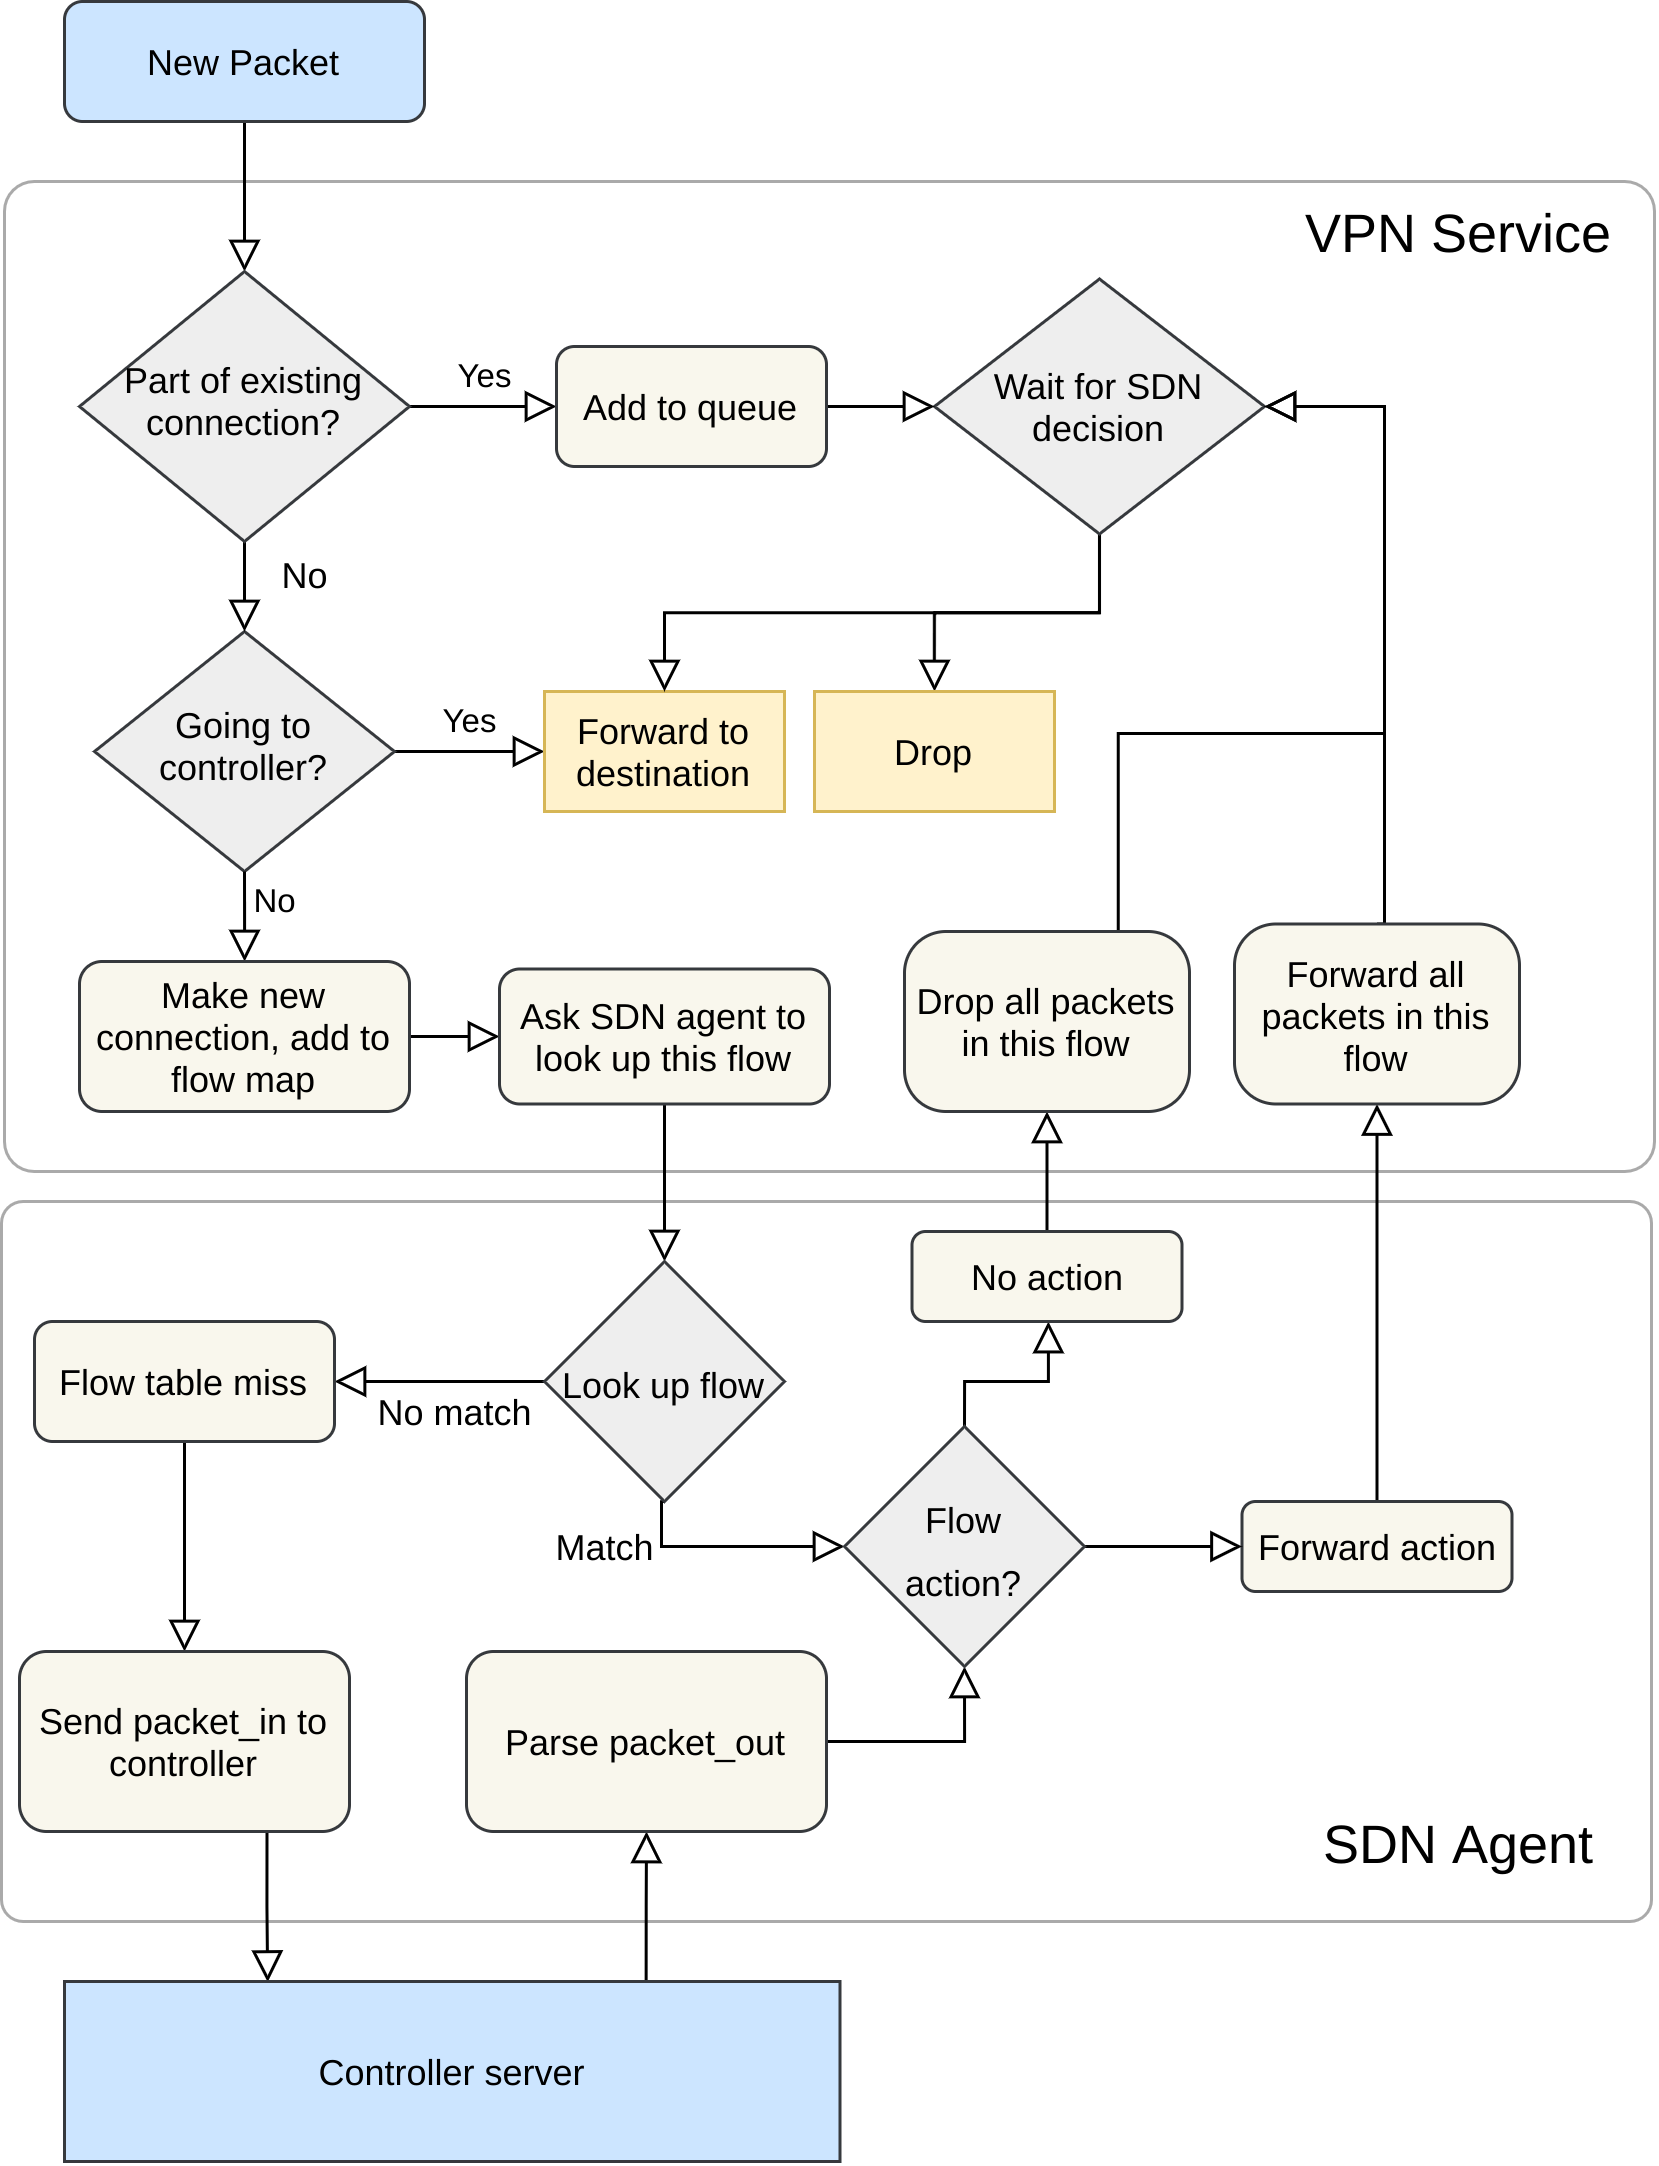
\includegraphics[width=\textwidth]{sequence-diagram.png}
    \caption{Flow chart of the steps used to decide whether to forward or drop a
		packet.}
    \label{fig:sequence-diagram}
\end{figure}

\subsubsection{OpenFlow Protocol}
\label{sec:openflow-protocol}

The OpenFlow Switch Specification describes a protocol for SDN agents to connect
to a controller and exchange messages. \textsc{Appjudicator} implements the
minimum allowable subset of this specification. All OpenFlow messages are sent
over TCP in OpenFlow packets. These packets have a simple 8-byte header that
describes the OpenFlow version, the type of the message, the total length of the
packet, and transaction ID (see Figure~\ref{fig:openflow-header}). Replies to an
OpenFlow message have the same transaction ID as the request.

\begin{figure}[h]
    \centering
    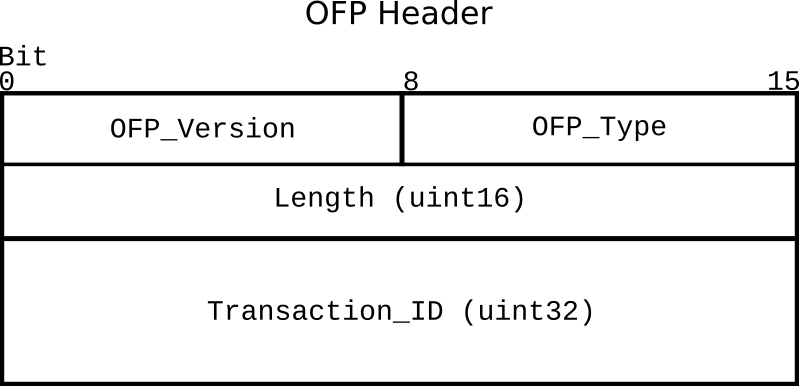
\includegraphics[width=.6\textwidth]{openflow-header.png}
    \caption{Fields of an OpenFlow packet header.}
    \label{fig:openflow-header}
\end{figure}

When the app is launched it opens a new TCP connection to a user-configurable IP
address or host name that runs the controller server. The controller and switch
each send a message of type \texttt{OFPT\_HELLO} to initiate the connection. The
controller then queries the switch to see what capabilities and features it
supports with a \texttt{OFPT\_FEATURES\_REQUEST}.  \textsc{Appjudicator} replies
with a message explaining that it has one physical port (the phone itself) and
only supports two packet actions: forward and drop.  At this point the
connection is fully established, and the controller and agent can both send
messages back and forth. Figure~\ref{fig:openflow-handshake} shows this process.

% TODO talk about how we only support a subset of normal flow table entries

\begin{wrapfigure}{R}{0.4\textwidth}
	\centering
	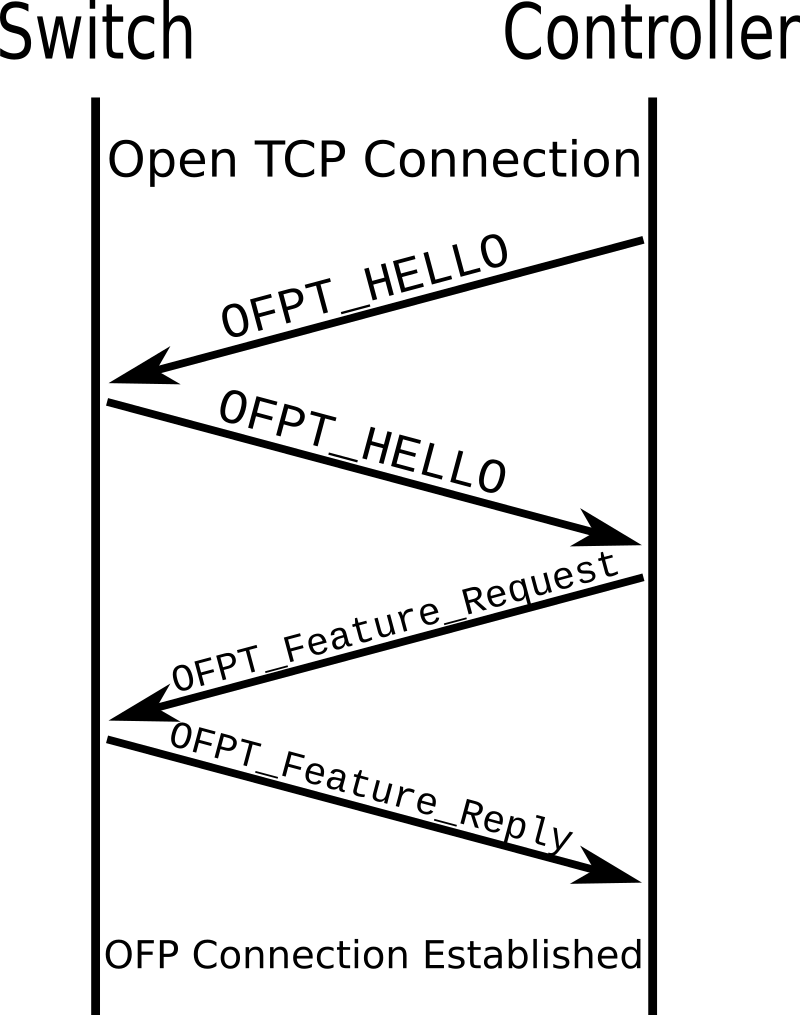
\includegraphics[width=0.4\textwidth]{openflow-handshake.png}
    \caption{OpenFlow handshake diagram.}
    \label{fig:openflow-handshake}
\end{wrapfigure}

% TODO add more about switch-initiated messages (packet-in and packet-out)

\subsubsection{Associating Network Flows with Context}
\label{sec:associating-network-flows-with-context}

\textit{[Details of this section may change.]}

When the SDN agent intercepts a new flow to a previously unknown domain, it
tries to associate it with UI context. The app looks up any accessibility events
that occurred in the two seconds before the flow was initiated. If there is no
likely initiator of the network flow (such as a button press) within the two
prior seconds the flow is considered non-user-initiated. The SDN agent includes
information about these UI events, including the event type and view hierarchy
(see Section~\ref{sec:identifying-ui-elements}) with the packet as it is
elevated to the controller. This UI context should allow for more powerful and
fine-grained SDN rules.

% TODO add more info here, stuff about getting PIDs

\subsubsection{Default-Allow Flows}
\label{sec:default-allow-flows}

Our system must account for non-user-initiated flows that occur as part of the
normal operation of the device. To do this, we profile the Android operating
system and common applications in advance.  While running in calibration mode,
\textsc{Appjudicator} adds the IP address and ports of all non-user-initiated
requests to a default-allow map. Then later, while operating normally, the app
will not question flows to these pairs of IP address and ports even if they are
not user-initiated.

% TODO add more info here

% TODO what to do when controller is unavailable

\newpage
